\documentclass[twocolumn]{jsarticle}
\usepackage{newtxtext}
\usepackage{float}
\usepackage{abstract}
\usepackage[dvipdfmx]{graphicx}
\usepackage{here}
\usepackage{subfigure}
\usepackage{graphicx}% Include figure files
\usepackage{dcolumn}% Align table columns on decimal point
\usepackage{bm}% bold math
\usepackage{lipsum}
\renewcommand{\abstractname}{要旨}

\begin{document}
\twocolumn[
\tableofcontents
]
\title{RNNを用いた自動車走行時の車両状態予測に関する研究}
\author{研究者 岩谷 燎\and 指導教員 加藤 聡}
\date{\today}

\twocolumn[
\maketitle
\begin{onecolabstract}
近年,自動車制御の分野において,予防安全技術の発展が著しい.しかし,車両制御の予防安全技術はセンサーから得る車両の走行情報から現時点での状態を判断,制御しているため完全な予防安全技術ではない.そこで本研究では,RNN(Recurrent Neural Network)を用いて現在の自動車の走行状態から,未来の走行状態を予測することを目的とした.
物理シミュレーションによって取得された車両の走行データを用いた学習実験の結果,限定的ではあるが,車両状態の予測が可能であることが分かった.

\noindent
\textbf{キーワード} 自動車,予防安全技術,車両制御,走行状態,RNN,予測
\end{onecolabstract}
]
%%%%%%%%%%%%%%%%%%%%%%%%%%%%%%%%%%%%%%%%%%%%%%%%%%%%%%%%%%%%%%%%%%%%%%%%%%%%%%%%%%%
\section{はじめに}
自動車制御の分野において,ここ数年で特に発展を遂げているのが,自動運転技術及び予防安全技術である.
しかし,車両制御の予防安全技術は,センサーから得る車両の情報からその時点での状態を判断し制御しているに過ぎず,
現在の自動車の操作,走行状態から,未来の状態を予測し,予防安全制御を行うには至っていない.
本研究では,現在の操作,走行状態から車両限界の直前で予防安全制御を行うまでの,未来の車両状態を予測判断するシステムを開発することを目的とする.
%%%%%%%%%%%%%%%%%%%%%%%%%%%%%%%%%%%%%%%%%%%%%%%%%%%%%%%%%%%%%%%%%%%%%%%%%%%%%%%%%%%
\section{車両制御による予防安全技術}
現在の車両制御の予防安全技術として,TRC(Traction Control)やVSC(Vehicle Stability Control),ABS(Anti-lock Brake System)などが挙げられる.TRCはタイヤのスリップを検知し,スリップしたタイヤのトルクを抑制したりブレーキをかけることにより適切な駆動力を確保しタイヤの空転を抑え,接地性を確保し車両の走行を安定させる技術である.VSCは車両の横滑りを検知し,4輪個々のブレーキの力とエンジン出力を自動制御し,車両の安定性を確保する技術である.
ABSはブレーキ時のタイヤのスリップによるロックを検知し,ブレーキ圧を緩めロックを解消させ,再度ブレーキ圧を高める,という制御を短時間で繰り返すことにより,ステアリング操作を容易にし,車両停止性を確保する技術である[9].
\\ これらの予防安全技術は,スリップや横滑りを検知してから車体を制御しているため,予防の観点からは完全であるとは言えない.
\begin{figure}[H]
	\centering
	\includegraphics[width=7cm]{trc.jpg}
	\caption{Traction Control}
	\label{fig01}
\end{figure}
\begin{figure}[H]
	\centering
	\includegraphics[width=7cm]{vsc.jpg}
	\caption{Vehicle Stability Control}
	\label{fig02}
\end{figure}
\begin{figure}[H]
	\centering
	\includegraphics[width=7cm]{abs.jpg}
	\caption{Anti-lock Brake System}
	\label{fig03}
\end{figure}
%%%%%%%%%%%%%%%%%%%%%%%%%%%%%%%%%%%%%%%%%%%%%%%%%%%%%%%%%%%%%%%%%%%%%%%%%%%%%%%%%%%
\section{自動車走行時の車両状態}
\subsection{概要}
本研究での自動車走行時の車両状態は舵角に対する車両の移動方向が異なる横滑りや,タイヤと路面間の滑りであるスリップを取り上げる.
\subsection{横滑り}
横滑りとは,タイヤの舵角と進行方向の差であるスリップ角の大きさにより発生する[5].スリップ角の概要図を図4に示す.
自動車は進行方向を変える際,タイヤの向きを変えるが,そのときタイヤは車体に対して平行な状態に戻ろうとする.
そのときに生じる力の反作用であるコーナリングパワー$K$と,スリップ角$β$によりコーナリングフォース$F$が与えられる.
   \begin{equation}
   \label{equation1}
      F = Kβ
   \end{equation}
$F$により車体は向きを変える.図5よりスリップ角が増加していくと,約4度までは線形領域であり,直線的にコーナリングフォースが増加していく.さらにスリップ角が大きくなると,非線形領域となり,増加割合は減少する.さらに大きいスリップ角域(約10 ~ 15度)では限界領域となり,飽和または減少傾向となり,滑り状態に遷移していく.この状態が横滑り状態と定義される[5].
\\ 横滑りはアンダーステア,オーバーステアに分類される.アンダーステア,オーバーステアの判定はスリップ角により判定する.スリップ角$β$は前輪,後輪それぞれ$β_f$,$β_r$に分けられる.
\\ アンダーステア,オーバーステアの定義については,$β_f > β_r \land β_f > 10$ の時がアンダーステアとし,$β_f < β_r \land β_r > 10$ の時がオーバーステアと定義される[5].
\\ それぞれの滑り状態の具体的な挙動については,アンダーステアは旋回しているとき,速度が上がるにしたがって車両の向きが外側に膨らんでいき.オーバーステアは旋回中に速度が上がるにしたがって車両の向きが内側に切れ込んでいく[5].アンダーステア,オーバーステア時の車体挙動の例を図6に示す.
\begin{figure}[H]
	\centering
	\includegraphics[width=8cm]{slip_angle.jpg}
	\caption{スリップ角の概要図}
	\label{fig04}
\end{figure}
\begin{figure}[H]
	\centering
	\includegraphics[width=7cm]{kf.jpg}
	\caption{タイヤのコーナリングフォース特性([5]より引用)}
	\label{fig05}
\end{figure}
\begin{figure}[H]
	\centering
	\includegraphics[width=7cm]{slip.jpg}
	\caption{横滑りの挙動例}
	\label{fig06}
\end{figure}
\subsection{スリップ}
スリップは四輪それぞれのスリップ率$S$により判定する.スリップ率は,制動時において,
   \begin{equation}
   \label{equation2}
      S = \frac{車両速度 - 車輪速度}{車両速度}
   \end{equation}
駆動時において,
   \begin{equation}
   \label{equation3}
      S = \frac{車輪速度 - 車両速度}{車輪速度}
   \end{equation}
と定義する.ここで車輪速度は,($タイヤの有効半径 \times タイヤ回転角速度$)を意味する.
\\ スリップの具体的な挙動として,スリップ率が0のときは車輪が全く滑らなく,スリップ率が1のとき,制動時は車輪がロックして車両が滑っている状態,駆動時は車輪が滑り全く進まない状態である[5].図7より,スリップ率が約0.2以上のとき,タイヤの横力が大幅に減少しているため,スリップ率が$S > 0.2$のときをスリップと定義する.本実験では少なくとも一つのタイヤのスリップ率が$S > 0.2$となった場合をスリップ状態とする.
\begin{figure}[H]
	\centering
	\includegraphics[width=7cm]{slipratio.jpg}
	\caption{スリップ率に対するタイヤの前後力,横力の特性([5]より引用)}
	\label{fig15}
\end{figure}
%%%%%%%%%%%%%%%%%%%%%%%%%%%%%%%%%%%%%%%%%%%%%%%%%%%%%%%%%%%%%%%%%%%%%%%%%%%%%%%%%%%
\section{RNN(Recurrent Neural Network)}
\subsection{概要}
RNNとは,NN(Neural Network)の隠れ層にフィードバック接続があり,ある時点での内部状態を次の状態の入力値として扱い,時系列に応じて異なる解を出力するNNである[4].RNNのが概要図を図8に示す.RNNにより,時系列データのパターンを認識することができ,過去のデータ系列から未来を予測した出力を出すことが可能となる.本研究でのRNNの中間層にはLSTM(後述)を使用する.
\begin{figure}[H]
	\centering
	\includegraphics[width=7cm]{RNNdef.PNG}
	\caption{RNNの概要図}
	\label{fig07}
\end{figure}
\subsection{LSTM(Long Short Term Memory)}
基本構成のRNNでは深いネットワークになると誤差逆伝播のアルゴリズムでは誤差関数の勾配の消失や発散などによる問題が生じてしまうため,時系列の長期依存性を正確に扱えない.LSTMはその問題を緩和したモデルである[4].具体的な構造としては,出力ゲート(Output Gate),入力ゲート(Input Gate),忘却ゲート(Forget Gate),記憶セル(Memory Cell)が組み込まれている.図9にLSTMブロックの内部構成を示す[4].

時刻$t$におけるLSTMブロックへの入力は$x_t$と時刻$t - 1$におけるLSTMブロックの出力$h_{t-1}$である$x_t$と$h_{t-1}$は以下の式で変換される(図10).
  \begin{equation}
   \label{equation4}
      \overline{z_t} = W_zx_t + R_zh_{t-1} + b_z
   \end{equation}
   \begin{equation}
   \label{equation5}
      z_t = \tanh (\overline{z_t})
   \end{equation}

入力ゲートにおける変換を以下に示す(図11).入力ゲートでは,必要な誤差信号のみを適切に伝播させるために前の時刻のデータ出力を受け取るか否かの判断を行う.
  \begin{equation}
   \label{equation6}
      \overline{i_t} = W_ix_t + R_ih_{t-1} + b_i
   \end{equation}
   \begin{equation}
   \label{equation7}
      i_t = σ(\overline{i_t})
   \end{equation}

忘却ゲートにおける変換を以下に示す(図12).忘却ゲートでは,誤差信号を受け取ることで記憶セルで記憶した内容を一度に忘却させ,入力系列のパターンが急激に変化したときに素早く記憶セルを初期化することを可能とする.
  \begin{equation}
   \label{equation8}
      \overline{f_t} = W_fx_t + R_fh_{t-1} + b_f
   \end{equation}
   \begin{equation}
   \label{equation9}
      f_t = σ(\overline{f_t})
   \end{equation}

記憶セルにおける変換を以下に示す(図13).式(\ref{equation10})の$c_{t-1}$は1つ前の時刻での記憶セルの出力である.記憶セルでは現在の出力を次の時刻の処理で使うために,一時的に記憶している.
  \begin{equation}
   \label{equation10}
      c_t = i_t \otimes z_t + f_t \otimes c_{t-1}
   \end{equation}

出力ゲートにおける変換を以下に示す(図14).出力ゲートも入力ゲートと同様に必要な信号のみを出力するための判断を行う.
  \begin{equation}
   \label{equation11}
      \overline{o_t} = W_ox_t + R_oh_{t-1} + b_o
   \end{equation}
   \begin{equation}
   \label{equation12}
      o_t = σ(\overline{o_t})
   \end{equation}

最後にLSTMブロックの出力部分の式が以下で示される(図15).
   \begin{equation}
   \label{equation13}
      y_t = h_t = o_t \otimes \tanh (c_t)
   \end{equation}

LSTMブロックへの入力である$x_t$の次元を$m$,出力である$y_t$の次元を$n$とする.$h_t$の次元も$n$となる.$W_z,W_i,W_f,W_o,$は$m \times n$の行列,$R_z,R_i,R_f,R_o$は$n \times n$の行列,$b_z,b_i,b_f,b_o$は$n$次元ベクトルのバイアスである.
\begin{figure}[H]
	\centering
	\includegraphics[width=7cm]{LSTM.jpg}
	\caption{LSTMブロックの中身([4]より引用)}
	\label{fig08}
\end{figure}

\begin{figure}[H]
	\centering
	\includegraphics[width=7cm]{input.jpg}
	\caption{$\overline{z_t}$と$z_t$([4]より引用)}
	\label{fig09}
\end{figure}

\begin{figure}[H]
	\centering
	\includegraphics[width=7cm]{input_gate.jpg}
	\caption{$\overline{i_t}$と$i_t$([4]より引用)}
	\label{fig010}
\end{figure}

\begin{figure}[H]
	\centering
	\includegraphics[width=7cm]{forget_gate.jpg}
	\caption{$\overline{f_t}$と$f_t$([4]より引用)}
	\label{fig11}
\end{figure}

\begin{figure}[H]
	\centering
	\includegraphics[width=7cm]{memory_cell.jpg}
	\caption{記憶セルにおける変換([4]より引用)}
	\label{fig12}
\end{figure}

\begin{figure}[H]
	\centering
	\includegraphics[width=7cm]{output_gate.jpg}
	\caption{$\overline{o_t}$と$o_t$([4]より引用)}
	\label{fig13}
\end{figure}

\begin{figure}[H]
	\centering
	\includegraphics[width=7cm]{output.jpg}
	\caption{LSTMブロックの出力([4]より引用)}
	\label{fig14}
\end{figure}

%%%%%%%%%%%%%%%%%%%%%%%%%%%%%%%%%%%%%%%%%%%%%%%%%%%%%%%%%%%%%%%%%%%%%%%%%%%%%%%%%%%
\section{提案手法}
\subsection{概要}
本研究では,自動車走行時に得られる舵角や速度等に関する時系列データを機械学習にかけて,学習結果を基に一定時間後の車両状態を予測するものである.時系列データを学習させる手法としてはRNN(Recurrent Neural Network)を用いる.
\subsection{予測手法}
時系列データの予測手法として,SARIMAモデルやRandomForest,RNNが挙げられる.SARIMAモデルは一定の周期で同程度の値の変動をしている定常過程に従うデータを扱うARMAモデルに非定常データとの差分を取り,定常データとして扱うARIMAモデルを発展させたもので,季節要素に対応した中長期的な変動要素にも対応する汎用的な予測モデルである[1],[8].また,RandomForestは段階的にデータを分割していき、木のような分析結果を出力する決定木モデルが基となる.複数の決定木モデルを足し合わせ,平均化するアンサンブル学習というアルゴリズムを利用したモデルで,決定木モデルより高性能な予測が可能となっている[2].
\\ SARIMAモデルは非定常過程データにも対応しているが,やはり周期的な要素を基に予測をしているため,自動車の運転という状況や時刻に応じて全く周期性の無いデータに対しては筆者の調査の範囲内では事例がない.Random Forestは分類にも回帰にも利用できる万能なモデルではあるが,時系列予測ではRNNの方が性能が良いため今回はRNNを選択した[3].
\subsection{提案手法の流れ}
具体的な提案手法の流れを以下に示す.本研究では現実世界で自動車を実際に走行させ,データを取得することが困難であるため,仮想空間上で自動車モデルを用いて研究を行う.

\begin{enumerate}
   \item 仮想空間を構築し,自動車モデルを用いて,一定時間毎の走行時のアクセル開度,舵角,速度,加速度,前輪スリップ角,後輪スリップ角,左前輪スリップ率,右前輪スリップ率,左後輪スリップ率,右後輪スリップ率の10種類の時系列データを取得する.
   \item 取得した時系列データをRNNに入力し,数秒前~現在の走行データの時系列の流れとそれによる一定時間後の前輪スリップ角,後輪スリップ角,左前輪スリップ率,右前輪スリップ率,左後輪スリップ率,右後輪スリップ率を学習させる.
   \item 学習したRNNに学習データ,テストデータを入力し,出力された前輪スリップ角,後輪スリップ角,左前輪スリップ率,右前輪スリップ率,左後輪スリップ率,右後輪スリップ率の予測時系列データを横滑りは3.2節,スリップは3.3節の条件をもとにデータを分類,学習データ,テストデータの教師データと比較する.
\end{enumerate}

%%%%%%%%%%%%%%%%%%%%%%%%%%%%%%%%%%%%%%%%%%%%%%%%%%%%%%%%%%%%%%%%%%%%%%%%%%%%%%%%%%%
\section{評価実験}
\subsection{学習データの作成}
本研究では,Unity[6]による仮想空間内に敷設されたコース(図16)を基軸に走行パターン(速度やアクセルの踏み具合,カーブの曲がり方,逆走等)を変更しながら自動車モデルを走行させ,0.12秒毎のアクセル開度,舵角,速度,加速度,前輪スリップ角,後輪スリップ角,左前輪スリップ率,右前輪スリップ率,左後輪スリップ率,右後輪スリップ率の10種類の時系列データを取得する.学習データでは600秒間(5000個),テストデータでは3600秒間(30000個)のデータを用意する.
教師データは0.6秒後の前輪後輪スリップ角,前後左右輪スリップ率の信号を用意する.
入力用時系列データは機械学習の効率化のため標準化(平均を0,分散を1とする)を行う[7].
\subsection{構築したRNNの概要}
構築するRNNはスリップ角,スリップ率の連続データを出力するモデルを作成する.
RNNの構造は,入力層の次元は10,中間層(LSTMブロック)の次元は128とする.出力はスリップ角の場合,前輪後輪それぞれスリップ角の連続データが存在するため次元は2,スリップ率では前後左右輪それぞれの連続データが存在するため次元は4とする.
学習時に時系列データを実際にRNNに入力するときは走行データを連続した10個(1.2秒)の時系列データと5個後(0.6秒後)の教師データを1つのミニバッチとし,入力するミニバッチ学習を行う.ミニバッチの具体例を図17に示す.ミニバッチは開始位置をデータ長5000から4950個重複の無いように変え,作成する.作成した4950個のデータをランダムに入力し,学習を行う.ここまでを1セットとし,学習を1000セット行う.モデルは学習10回毎に保存する.

\onecolumn
\begin{figure*}[tbp]
	\centering
	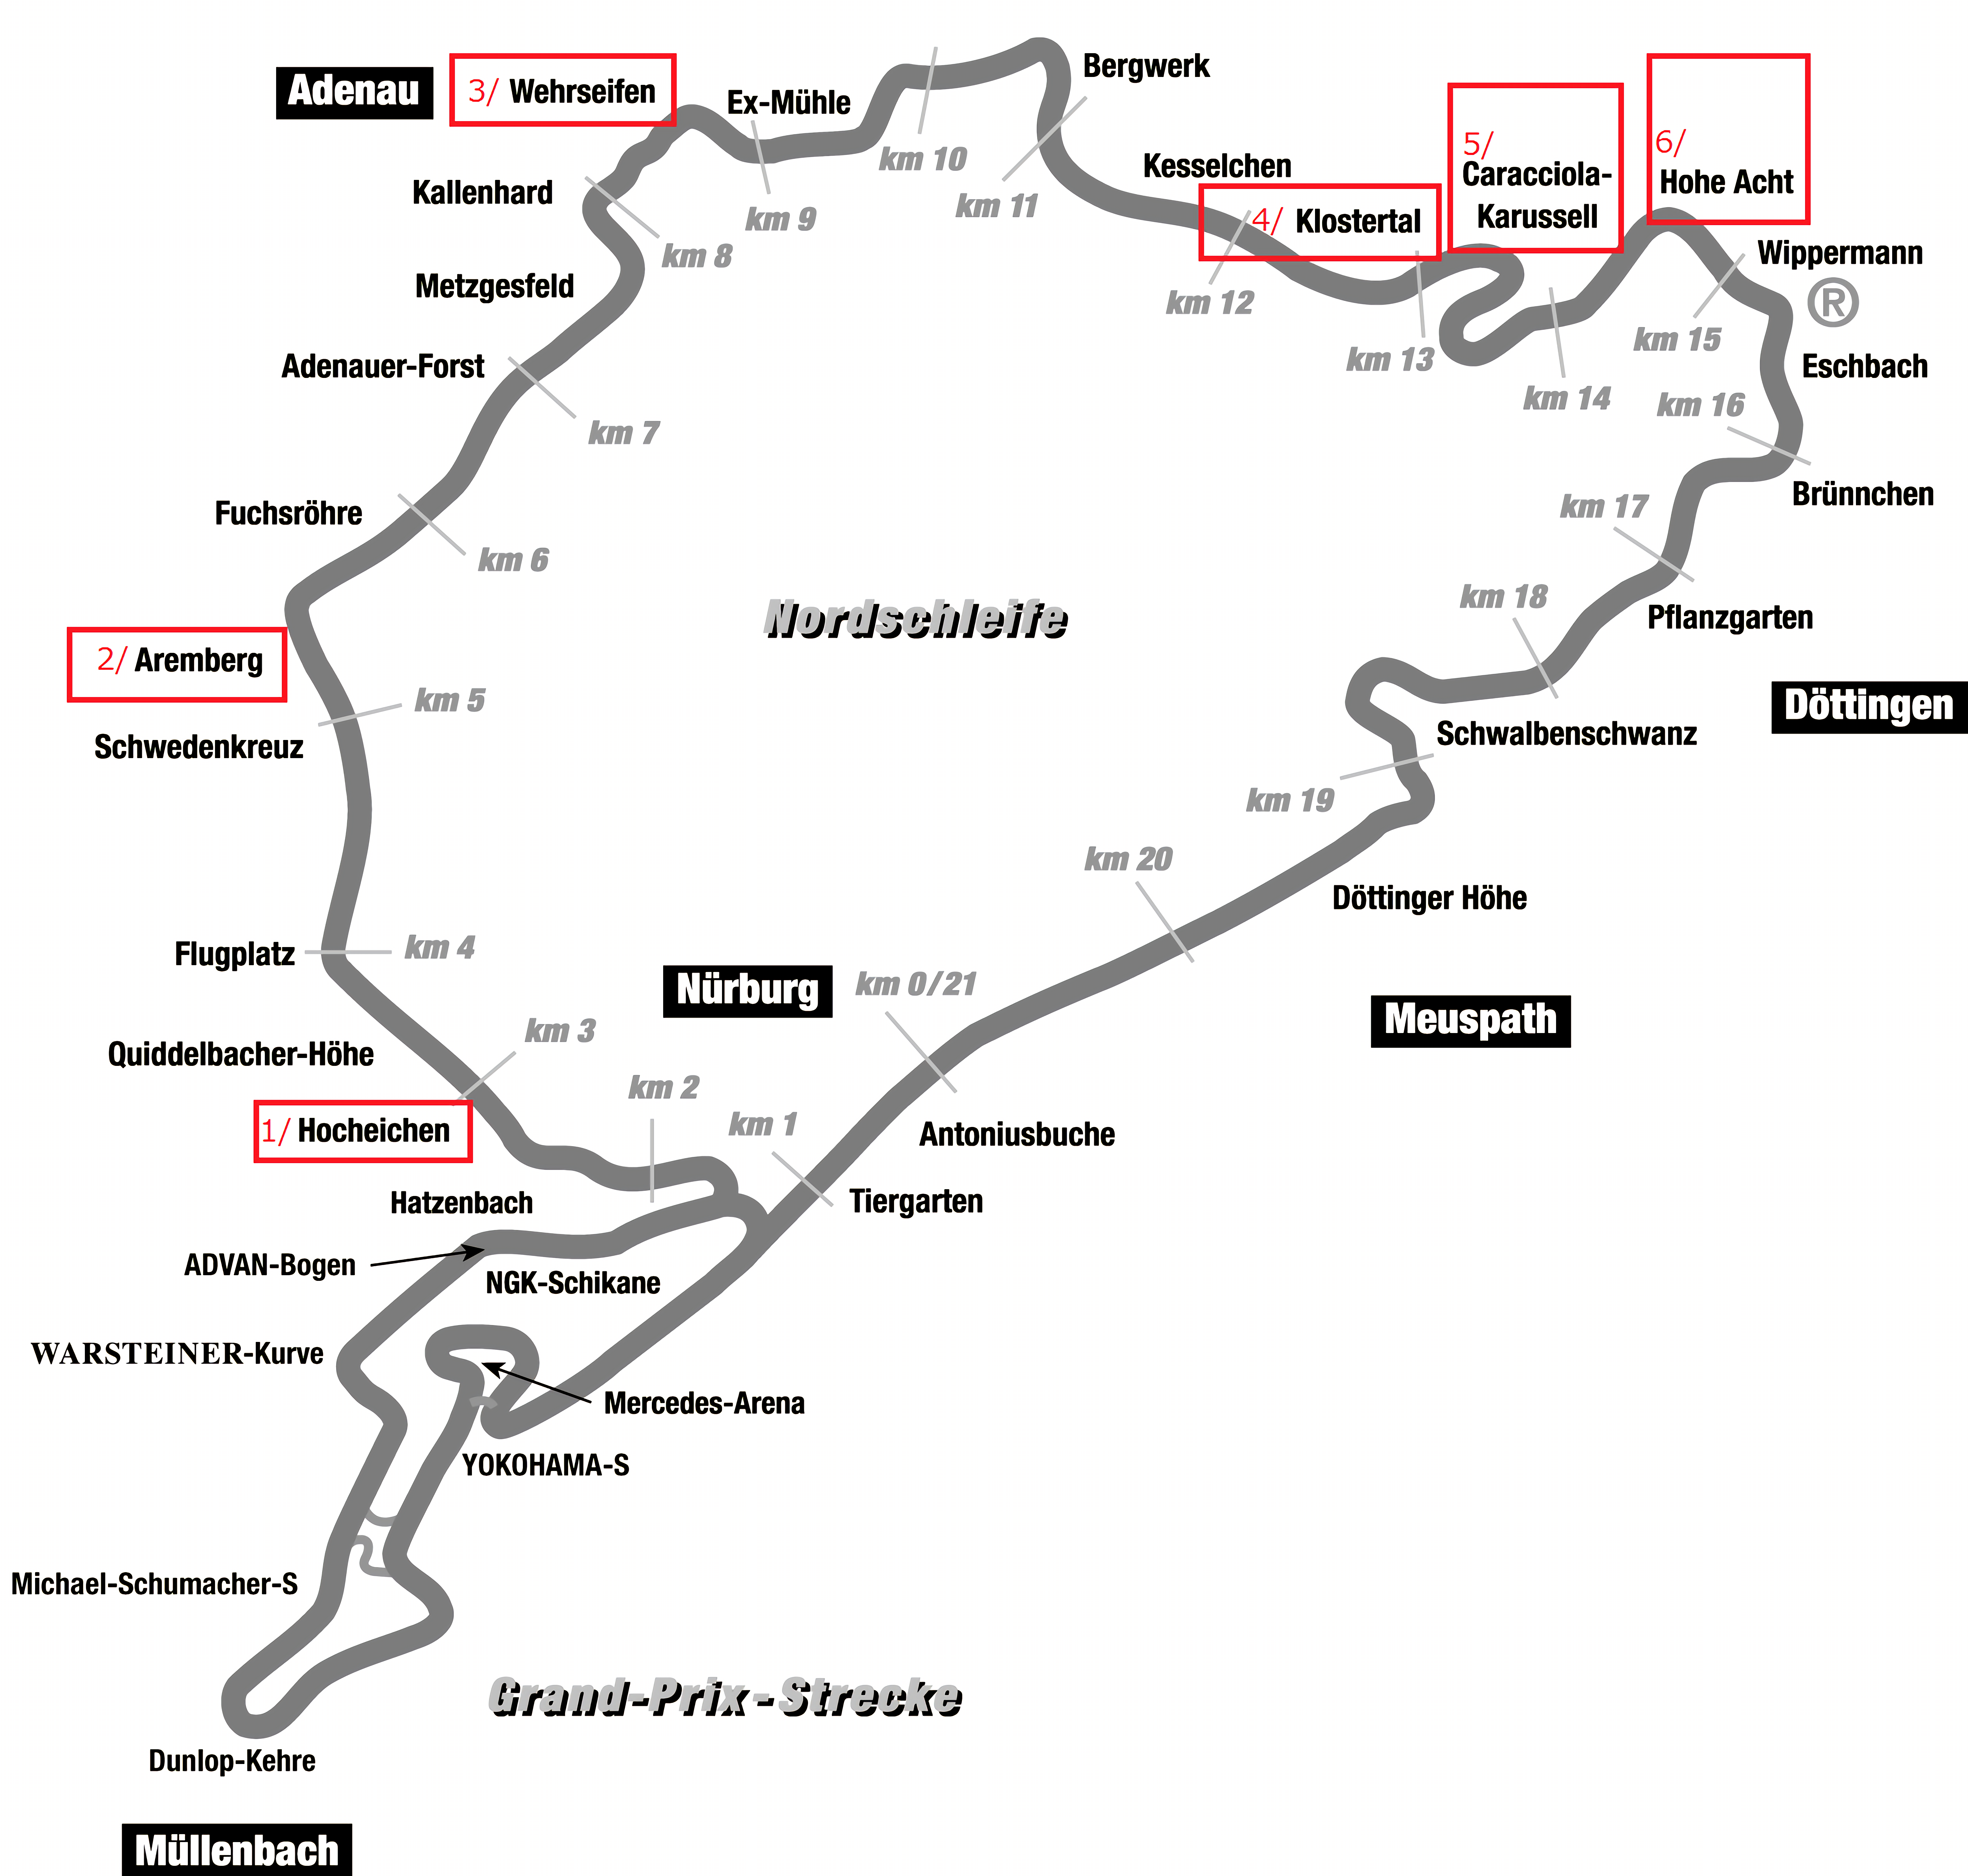
\includegraphics[width=12cm]{Nordschleife.PNG}
	\caption{コース図([13]より引用)}
	\label{fig17}
\end{figure*}
\begin{figure*}[tbp]
	\centering
	\includegraphics[width=12cm]{minibatch.PNG}
	\caption{ミニバッチの具体例}
	\label{fig18}
\end{figure*}
\twocolumn



\subsection{実験内容}
上記の学習内容に基づき構築された10回毎の学習回数ごとのRNNの,
学習データとテストデータに対する予測データの分類を行う.
横滑りは3.2節の条件下でのアンダーステア,オーバーステアと,
通常走行の3状態とする.
分類する際,アンダーステアは1,
オーバーステアは-1,
通常走行は0を与える.
スリップについても3.3節の条件下でスリップ状態,非スリップ状態とする.
スリップ状態で1,非スリップ状態で0を与える.

以上の条件に基づき,学習データ,テストデータ,予測データをデータ整形する.具体的には,横滑りの場合,時系列データの各時刻の前輪後輪スリップ角が$β_f > β_r \land β_f > 10$のとき1を,$β_f < β_r \land β_r > 10$のとき-1,それ以外では0と整形する.スリップの場合,各時刻の前後左右輪スリップ率が少なくとも一つが$S > 0.2$とのとき1を,そうでなければ0となるよう整形する.具体例として学習データを整形したグラフを図\ref{fig24}に示す.
整形後のデータはテストデータと予測データ間の予測精度を全ての走行状態に対する精度の高さを算出するため,マクロ平均によるF値により評価を行う.
F値とは,$i(i = 1,2,...,N)$クラスの分類問題を考えたとき,$i$と予測したデータのうち,実際に$i$であるものの割合である適合率$P_i$と実際に$i$であるもののうち,$i$であると予測された者の割合である再現率$R_i$をもちいて
   \begin{equation}
   \label{equation14}
      F_i = \frac{2R_i \cdot P_i}{R_i+P_i}(i = 1,2,...,N)
   \end{equation}
と表せる[8],[9]..この$F_i$は各クラスにおけるF値である.そのため全体のF値$F_{total}$を求める必要があるが,本研究ではマクロ平均を用いる.マクロ平均とはNセットのテストをする場合に,各セットで評価値を計算した後,それらを平均する手法である[8],[10].マクロ平均を用いると$F_{total}$は
   \begin{equation}
   \label{equation15}
     F_{total} = \frac{1}{N}\sum_{i=1}^N F_i
   \end{equation}
で表す.本研究では横滑りは(-1,0,1)の3クラス,スリップは(0,1)の2クラスの分類問題とし,式\ref{equation14},\ref{equation15}を用いてマクロ平均によるF値を計算する.



\subsection{結果}
上記の学習内容に基づき分類構築されたRNNの,学習回数ごとの学習データとテストデータに対する予測データのF値の関係を図\ref{fig19}に,最もテストデータに対するF値が高かったグラフの波形を図\ref{fig20}~図\ref{fig23}に,データ整形後のF値の表を表\ref{table01}に示す.図\ref{fig20}~図\ref{fig23}は実線が教師データ,破線が予測データである.最もテストデータに対するF値が高かった学習回数は,横滑り予測モデルは80回,スリップ予測モデルは30回であった.しかし,最もテストデータに対して高かったF値が横滑りでは約0.48,スリップでは約0.58と低い値であった.また,学習データに対しても,横滑りでは0.65,スリップでは0.59とテストデータに対するF値より高い値ではあるものの,やはり低い値にとどまった.
図\ref{fig20}~図\ref{fig23}のグラフ波形については,学習データに対しては横滑り,スリップ共に,教師データに対して高い追随性を持っていた.テストデータについても,教師データの急激な値の増減に追随しきれていなかったり,位相が少しずれている箇所も見受けられるが,グラフの特徴はうまく捉えられていることが確認された.

\subsection{考察}
図\ref{fig20}~図\ref{fig23}のように,テストデータ,学習データ共に教師データに対して高い追随性を持っているにも関わらず,表\ref{table01}から車両状態予測のF値が低い値であった原因として,横滑りでは前輪スリップ角,後輪スリップ角の大小関係が教師データと予測データで逆転していることや,僅かな位相のずれが,全く異なる車両状態を予測してしまう,といったことが考えられる.スリップについては横滑りと同様に,位相のずれによる車両状態の誤認識が挙げられるが,他に,スリップ率がスリップ状態判定の閾値である0.2付近での教師データに対して,予測データが微少な値の増減に追随しきれなかったことが考えられる.
また,図\ref{fig19}のように,学習回数が増加していくに従い,テストデータに対するF値が減少していく原因として,学習データに対する学習の停滞が考えられる.

\onecolumn
\begin{figure*}[tbp]
	\centering
	\subfigure[横滑りの分類(整形)]{\includegraphics[width=12cm]{spin_classification.png}}\\
	\subfigure[スリップの分類(整形)]{\includegraphics[width=12cm]{slip_classification.png}}
	\caption{データ分類(整形)後の学習データ}
	\label{fig24}
\end{figure*}
\begin{figure*}[tbp]
	\centering
	\subfigure[横滑り予測]{\includegraphics[width=14cm]{spin_f.PNG}}\\
	\subfigure[スリップ予測]{\includegraphics[width=14cm]{slip_f.PNG}}
	\caption{予測データのF値}
	\label{fig19}
\end{figure*}
\begin{figure*}[tbp]
	\centering
	\subfigure[前輪スリップ角]{\includegraphics[width=11cm]{train_front_tire_slipangle.png}}\\
	\subfigure[後輪スリップ角]{\includegraphics[width=11cm]{train_rear_tire_slipangle}}
	\caption{学習データに対するスリップ角の予測グラフ}
	\label{fig20}
\end{figure*}

\begin{figure*}[tbp]
	\centering
	\subfigure[前輪スリップ角]{\includegraphics[width=11cm]{test_front_tire_slipangle.png}}\\
	\subfigure[後輪スリップ角]{\includegraphics[width=11cm]{test_front_tire_slipangle.png}}
	\caption{テストデータに対するスリップ角の予測グラフ}
	\label{fig21}
\end{figure*}

\begin{figure*}[tbp]
	\centering
	\subfigure[左前輪スリップ率]{\includegraphics[width=12cm]{train_front_left_slipratio.png}}\\
	\subfigure[右前輪スリップ率]{\includegraphics[width=12cm]{train_front_right_slipratio.png}}\\
	\subfigure[左後輪スリップ率]{\includegraphics[width=12cm]{train_rear_left_slipratio.png}}\\
	\subfigure[右後輪スリップ率]{\includegraphics[width=12cm]{train_rear_right_slipratio.png}}
	\caption{学習データに対するスリップ率の予測グラフ}
	\label{fig22}
\end{figure*}

\begin{figure*}[tbp]
	\centering
	\subfigure[左前輪スリップ率]{\includegraphics[width=12cm]{test_front_left_slipratio.png}}\\
	\subfigure[右前輪スリップ率]{\includegraphics[width=12cm]{test_front_right_slipratio.png}}\\
	\subfigure[左後輪スリップ率]{\includegraphics[width=12cm]{test_rear_left_slipratio.png}}\\
	\subfigure[右後輪スリップ率]{\includegraphics[width=12cm]{test_rear_right_slipratio.png}}
	\caption{テストデータに対するスリップ率の予測グラフ}
	\label{fig23}
\end{figure*}
\begin{table*}[tbp]
   \caption{最も精度の高いF値}
   \label{table01}
   \begin{center}
   \begin{tabular}{|c||c|c|}\hline
                    & 学習データに対するF値 & テストデータに対するF値 \\ \hline
     横滑り予測 & 0.652386534 & 0.481942677 \\ \hline
     スリップ予測 & 0.590743774 & 0.575325588 \\ \hline
   \end{tabular}
   \end{center}
\end{table*}
\twocolumn
%%%%%%%%%%%%%%%%%%%%%%%%%%%%%%%%%%%%%%%%%%%%%%%%%%%%%%%%%%%%%%%%%%%%%%%%%%%%%%%%%%%
\section{まとめ}
本研究では,RNNによる深層学習を用いて,過去~現在の自動車走行時の車両状態から,未来の車両状態を予測することを試みた.スリップ角,スリップ率の予測までは高い追随性を持って可能であることが確認できたが,実際に車両状態をスリップ角,スリップ率から予測することは精度が低く,今後も検証の必要があると言える.今後の課題として予測精度の向上のため,RNNの学習パラメータの最適化,RNNの大型,複雑化,走行データ,バッチファイルの改善が挙げられる.
%以下,参考文献を書く部分
%件数が10を超える場合は,{9}の部分を{99}に変える.

\begin{thebibliography}{99}
%
\bibitem{sarima_ex}川崎智也,松田琢磨,花岡伸也:
  \newblock 「東アジア積米国揚コンテナ荷動き予測におけるSARIMAモデルの適用性」,
  \newblock 日本物流学会誌第21号,
  \newblock pp.167-174,
  \newblock 2013.5
%
\bibitem{random_forest}波部斉:
  \newblock 「ランダムフォレスト」,
  \newblock 情報処理学会研究報告,
  \newblock vol.2012-CVIM-182 No31,pp.1--8,
  \newblock 2012.5
%
\bibitem{randomforest_ex}宮崎邦洋,松尾豊:
  \newblock 「深層学習を用いた株価予測の分析」,
  \newblock The 31st Annual Conference of the Japanese Society for Artificial Intelligence, 2017
  \newblock pp.1-3,
  \newblock 2017
%
\bibitem{rnn}新納浩幸:
  \newblock Chainerによる実践深層学習,
  \newblock オーム社,
  \newblock pp.78--97,
  \newblock 2016.
%
\bibitem{car}野崎博路:
  \newblock 基礎自動車工学,
  \newblock 東京電機大学出版局,
  \newblock pp.1--38,
  \newblock 2008.
%
 \bibitem{unity}Unity:\\
  \newblock https://unity3d.com/jp
%
 \bibitem{fs}Importance of feature scaling:\\
  \newblock scikit-learn,\\
  \newblock scikit-learn.org/stable/auto\_examples/preprocessing\\
  \newblock /plot\_scaling\_importance.html
%
\bibitem{f1_score}sklearn.metrics.f1\_score:\\
  \newblock scikit-learn,\\
  \newblock scikit-learn.org/stable/modules/generated/sklearn.metrics.f1\_score.html
%
\bibitem{F}F値:\\
  \newblock 朱鷲の社Wiki,\\
  \newblock http://ibisforest.org/index.php?F値
%
\bibitem{macro}マクロ平均:\\
  \newblock 朱鷲の社Wiki,\\
  \newblock http://ibisforest.org/index.php?マクロ平均
%
\bibitem{sarima}未来を予測するビッグデータの解析手法と「SARIMAモデル」:\\
  \newblock DeepAge,\\
  \newblock https://deepage.net/bigdata/2016/10/22/bigdata-analytics.html
%
\bibitem{sarima}テクノロジーファイル 安全技術版:\\
  \newblock TOYOTA,\\
  \newblock https://www.toyota.co.jp/jpn/tech/safety\\
  \newblock /technology/technology\_file/active\_safety/
%
\bibitem{nuerburg}ニュルブルクリンク北コース画像を1967年と2014年で比べてみよう:\\
  \newblock http://dougarider.com/archives/34622\\
\end{thebibliography}

\end{document}